\section[Morphismen]{Morphismen und Isomorphismen von Spielen}\label{sec:Morphismen}

Wie wir im vorherigen Kapitel gesehen haben definieren Potentiale ein Koordinationsspiel, welches in einer \glqq gewissen Beziehung\grqq{} zu dem Ausgangsspiel steht (etwa die gleichen Nash-Gleichgewichte besitzt). Diese Beziehung wollen wir nun mit Hilfe eines Morphismus bzw. eines Isomorphismus zwischen den beiden Spielen präziser beschreiben. Die Eigenschaften, die Ausgangs- und Koordinationsspiel gemeinsam haben, sind dann genau die, die von den jeweiligen (Iso-)Morphismen bewahrt werden. Umgekehrt ist es auch möglich zuerst eine bestimmte Art von Isomorphimus zu definieren und daraus dann einen neuen Potentialbegriff zu erhalten wie das beispielsweise in \cite[Definitionen 5/6]{BestRespEq} getan wird.

Darüber hinaus helfen Morphismen dabei auch andere Beziehungen zwischen verschiedenen Spielen zu verstehen. Beispielsweise wird die von \citeauthor{MonShap} gefundene Äquivalenz von Auslastungsspielen und Spielen mit exaktem Potential durch einen passenden Isomorphiebegriff beschrieben und in \Cref{sec:Auslastungsspiele} werden wir noch weitere Beispiele für derartige Verbindungen kennenlernen. Schließlich ist es aus kategorientheoretischer Sicht auch allgemein wichtig die Morphismen der Kategorie, in der man arbeitet, zu verstehen, da diese die Struktur dieser Kategorie festlegen und etwa dazu verwendet werden abstrakte Konstruktionen durchzuführen. Diesen Ansatz werden wir hier allerdings nicht fortführen und verweisen dazu auf \cite{LapGameCat}.

\subsection{Definitionen}

\begin{defn}\label{defn:MorphismusVonSpielen}
	Zu zwei gegebenen Spielen $\Gamma = (I, X, (c_i)_{i\in I})$ und $\Delta = (J, Y, (d_j)_{j\in J})$ kann man wie folgt einen \emph{Morphismus} $(\sigma, \phi): \Gamma \to \Delta$ zwischen diesen beiden definieren:
	\begin{itemize}
		\item Eine Abbildung $\sigma: J \to I$ zwischen den Spielermengen, die \emph{Spielerabbildung}, und
		\item für jeden Spieler $j \in J$ eine Abbildung $\phi_j: X_{\sigma(j)} \to Y_j$ seiner Strategien, die \emph{Strategieabbildungen}.
	\end{itemize}
	Ist $(\tau, \psi): \Delta \to \Epsilon$ ein weiterer Morphismus, so ist die Verknüpfung der beiden Morphismen $(\sigma, \phi) \circ (\tau, \psi): \Gamma \to \Epsilon = (K, Z, (e_k)_{k \in K})$ gegeben durch
	\begin{itemize}
		\item die Spielerabbildung $\sigma\circ\tau: K \to I$ und
		\item die Strategieabbildungen $\psi_k \circ \phi_{\tau(k)}: X_{\sigma(\tau(k))} \to Z_k$.
	\end{itemize}
	$(\sigma, \phi)$ heißt \emph{Isomorphismus von Spielen}, wenn er einen inversen Morphismus besitzt, d.h. einen Morphismus $(\tau, \psi): \Delta \to \Gamma$ mit $(\sigma, \phi) \circ (\tau, \psi) = (\id, \id)$ und $(\tau, \psi) \circ (\sigma, \phi) = (\id, \id)$, wobei $(\id, \id)$, der Identitätsmorphismus auf dem jeweiligen Spiel, durch die Identität als Spielerabbildung und Identitäten für alle Strategieabbildungen gegeben ist.
\end{defn}

Diese Art und Weise Abbildungen zwischen zwei Spielen zu definieren ergibt sich aus dem - noch deutlich allgemeineren - Ansatz hierzu von \citeauthor{LapGameCat} in \cite{LapGameCat}\footnote{\citeauthor{LapGameCat} lässt in seiner Definition allerdings alle beteiligten Abbildungen in die jeweils umgekehrte Richtung gehen. Wir betrachten hier also gewissermaßen die zur dort definierten duale Kategorie.}. Wir orientieren uns dabei vor allem an dem dort in Kapitel 4 vorgestellten Morphismusbegriff für topologische Spiele (in denen die Spielermenge ein topologischer Raum und der Strategieraum eine Garbe über diesem ist) bzw. dessen Spezialisierung für Spiele für diskrete Spielermengen aus Kapitel 5. 

In dortigen Kontext ergibt es sich etwas natürlicher, dass die Abbildung zwischen den Spielermengen in die entgegengesetzte Richtung zu denen zwischen den Strategieräumen verläuft. Eine andere, auch im hier vorliegenden Kontext sinnvolle Begründung hierfür liefert aber die folgende Bemerkung:

\begin{bem}
	Alle Strategieabbildungen $\phi_j$ zusammen induzieren eine \emph{Strategieprofilabbildung}
	\[\phi: X \to Y: x=(x_i)_{i\in I} \mapsto \phi(x) := \left(\phi_j(x_{\sigma(j)})\right)_{j \in J} \]
\end{bem}

Würde die Abbildung $\sigma$ zwischen den Spielermengen in die andere, \glqq natürlichere\grqq{} Richtung verlaufen (also von $I$ nach $J$), so müssten wir zusätzlich fordern, dass diese bijektiv ist, damit in der obigen Form Strategieprofile auf Strategieprofile abgebildet werden (vgl. etwa \cite{CatGameTheory}). Denn nur dann wäre $\phi(x) \coloneqq \left(\phi_i(x_i)\right)$ wieder ein vollständiges und wohldefiniertes Strategieprofil in $Y$.

\begin{bem}
	Möchte man Spieler- und Strategieabbildungen in die gleiche Richtung haben und trotzdem Morphismen zwischen Spielen mit unterschiedlich großen Spielermengen erlauben, so kann man einem alternativen Ansatz zur Definition von Morphismen von Spielen folgen, welcher von \citeauthor{Foundations} in \cite[Kapitel 1, Abschnitt 1.14]{Foundations} verwendet wird: Hierbei wird als Spielerabbildung eine mengenwertige Abbildung verwendet, die also einen einzelnen Spieler nicht zwangsläufig wieder auf einen einzelnen Spieler abgebildet, sondern gleich auf eine ganze Teilmengen der Bildspielermenge. Von diesem Morphismentyp werden dann verschiedene \glqq approximativ kostenerhaltende\grqq{} Varianten betrachtet und die sich dadurch ergebende Kategorie untersucht.
\end{bem}

\begin{notation}
	In den meisten Fällen wird die Abbildung zwischen den Spielermengen allerdings doch bijektiv sein. In diesen Fällen werden wir zur Vereinfachung der Notation ohne Einschränkung davon ausgehen, dass die Spielermengen beider an der Abbildung beteiligten Spiele bereits gleich und geeignet permutiert sind, sodass $\sigma$ die Identitätsabbildung ist. Damit kann diese in der Notation weggelassen werden und die Abbildung zwischen den Spielen besteht nur noch aus den Abbildungen $\phi_i: X_i \to Y_i$ zwischen den Strategieräumen.
\end{notation}

Morphismen der in \Cref{defn:MorphismusVonSpielen} beschriebenen Form nehmen noch keinerlei Rücksicht auf die Kostenfunktionen der jeweiligen Spiele. Da gerade diese aber in der Regel die interessierenden Eigenschaften eines Spiels (wie beispielsweise Gleichgewichte) festlegen, werden derartige Abbildungen im Allgemeinen noch wenig Aussagen über die beteiligten Spiele ermöglichen. So besagt der durch diese Art Abbildungen induzierte Isomorphiebegriff bspw. nur, dass zwei Spiele Spieler- und Strategiemengen gleicher Kardinalität besitzen.

Sinnvollerweise sollten Morphismen zwischen Spielen folglich noch mehr der Struktur eines Spiels erhalten, insbesondere in irgendeiner Form \glqq verträglich\grqq{} mit den Kostenfunktionen sein. Je nach dem, welche Eigenschaften die Morphismen (und insbesondere die dadurch induzierten Isomorphismen) erhalten sollen, erhält man so unterschiedlich starke Verträglichkeitsbedingungen. Einige Möglichkeiten dafür werden wir nun kennenlernen.

Eine relative starke Forderung ist die, dass Morphismen \emph{kostenerhaltend} sein müssen, wie sie etwa in \cite[Abschnitt 2.1]{ReprOfFiniteGamesAsNCG} gestellt wird:

\begin{defn}
	Ein Morphismus $(\sigma, \phi_j)$ von $\Gamma = (I, X, (c_i)_{i\in I})$ nach $\Delta = (J, Y, (d_j)_{j\in J})$ heißt \emph{kostenerhaltend}, wenn für alle Strategieprofile $x \in X$ und jeden Spieler $j \in J$ gilt:
		\[c_{\sigma(j)}(x) = d_j(\phi(x)) \]
	Ist ein solcher Morphismus gleichzeitig ein Isomorphismus, so nennen wir $\Gamma$ und $\Delta$ \emph{äquivalent}.
\end{defn}

\begin{bem}
	Zwei Spiele sind also genau dann äquivalent, wenn sie sich ausschließlich durch Umbenennung der Strategien ineinander überführen lassen. In \cite[S. 133]{MonShap} wird dies als Isomorphie von Spielen bezeichnet.
\end{bem}

\begin{bsp}\label{bsp:Koordinationsspiel}
	Ein Spiel $\Delta = (J, Y, (d_j)_{j \in J})$ ist genau dann ein Koordinationsspiel, wenn es einen kostenerhaltenden Morphismus mit surjektiver Strategieprofilabbildung von einem 1-Personenspiel nach $\Delta$ gibt.
	
	Ist nämlich $\Delta$ ein Koordinationsspiel, so definiert man ein 1-Personenspiel $K \coloneqq (\{\ast\}, X, (c_\ast))$ mit $X = X_\ast \coloneqq Y$ und $c_\ast(y) \coloneqq d_{\hat{\jmath}}(y)$ für einen beliebigen, aber festen Spieler $\hat{\jmath} \in J$. Ferner definiert man den folgenden Morphismus $(\sigma, \phi): K \to \Delta$:
	\begin{align*}
		\sigma:	&&J		\to	 \{\ast\}:	&&j	\mapsto	\ast  \\
		\phi_j:	&&X_\ast	\to	 Y_j:	&&y	\mapsto	y_j
	\end{align*}	
	Dieser ist kostenerhaltend, denn für jedes Strategieprofil $y \in X = Y$ und jeden Spieler $j \in J$ gilt:
	\[c_{\sigma(j)}(y) = c_\ast(y) = d_{\hat{\jmath}}(y) \overset{\Gamma \text{ Koord.spiel}}{=} d_j(y) = d_j(\phi(y))\]
	Zudem ist offenbar die Strategieprofilabbildung $\phi$ surjektiv.
	
	Sind umgekehrt ein 1-Personenspiel $K = (\{\ast\}, X, (c_\ast))$ sowie ein kostenerhaltender Morphismus  $(\sigma, \phi): K \to \Delta$ mit surjektiven Strategieabbildungen gegeben, dann ist $\Delta$ bereits ein Koordinationsspiel. Denn aufgrund der Surjektivität von $\phi$ gibt es zu jedem Strategieprofil $y \in Y$ ein Strategieprofil $x \in X$ mit $\phi(x) = y$. Da $(\sigma, \phi)$ außerdem kostenerhaltend ist, folgt dann für je zwei Spieler $j, \hat{\jmath} \in J$: 
		\[d_{\hat{\jmath}}(y) = d_{\hat{\jmath}}(\phi(x)) = c_{\sigma(\hat{\jmath})}(x) = c_\ast(x) = c_{\sigma(j)}(x) = d_j(\phi(x)) = d_j(y)\]
	Also ist $\Gamma$ tatsächlich ein Koordinationsspiel.
\end{bsp}

Dieses Beispiel formalisiert die Intuition, dass in einem Koordinationsspiel alle Spieler ein gemeinsames Ziel haben und daher zusammen \glqq wie ein Spieler\grqq{} spielen (d.h. das Koordinationsspiel kann durch ein 1-Personenspiel simuliert werden).

%\begin{bsp}.
%	
%	\todo[inline]{Kann man auch Dummy-Spiele auf derartige Weise beschreiben?}
%\end{bsp}

In \cite{LapGameCat} stellt \citeauthor[Definition 4.1]{LapGameCat} folgende schwächere Verträglichkeitsbedingung:

\begin{defn}
	Ein Morphismus $(\sigma, \phi_j)$ von $\Gamma = (I, X, (c_i)_{i\in I})$ nach $\Delta = (J, Y, (d_j)_{j\in J})$ zusammen mit monotonen \emph{Kostenabbildung} $f_j: \IR \to \IR$ für jeden Spieler $j \in J$ heißt \emph{monoton}, wenn für jeden Spieler das folgende Diagramm kommutiert:	
	\begin{center}
		\begin{tikzcd}
			X \arrow[r, "\phi"] \arrow[d, "c_{\sigma(j)}"] 	& Y \arrow[d, "d_j"] \\
			\IR \arrow[r, "f_j"]							& \IR
		\end{tikzcd}
	\end{center}
	Ein solcher Morphismus heißt \emph{monotoner Isomorphimus}, wenn er ein Isomorphismus ist und auch die Verknüpfung der Kostenabbildungen die Identität gibt.
\end{defn}

\begin{bem}
	Gibt es eine derartige Abbildung $f_j$ für einen Spieler $j \in J$, so gilt für je zwei Strategieprofile $x, \hat{x} \in X$:
		\begin{align}\label{eq:CharExMonMor}
			c_{\sigma(j)}(x) \leq c_{\sigma(j)}(\hat{x}) \implies d_j(\phi(x)) \leq d_j(\phi(\hat{x}))
		\end{align}
	Ist umgekehrt diese Bedingung für je zwei Strategieprofile eines Spielers $j \in J$ erfüllt und zudem $d_j(\phi(X)) \subseteq \IR$ beschränkt oder $c_{\sigma(j)}(X) \subseteq \IR$ in beide Richtungen unbeschränkt, so gibt es eine solche Abbildung $f_j$.
\end{bem}

\begin{proof}
	Existiert eine Abbildung $f_j$, so gilt für zwei Strategieprofile $x, \hat{x} \in X$ mit $c_{\sigma(j)}(x) \leq c_{\sigma(j)}(\hat{x})$:
		\[d_j(\phi(x)) = f_j\circ c_{\sigma(j)}(x) \leq f_j\circ c_{\sigma(j)}(\hat{x}) = d_j(\phi(\hat{x}))\]
		
	Ist $d_j(\phi(X)) \subseteq \IR$ beschränkt oder $c_{\sigma(j)}(X) \subseteq \IR$ in beide Richtungen unbeschränkt, so können wir folgende Abbildung $f_j: \IR \to \IR$ definieren:
		\[f_j: \IR \to \IR: t \mapsto \begin{cases}
			\sup \Set{d_j(\phi(x)) | x \in X},								&\not\exists x \in X: c_{\sigma(j)}(x) \geq t \\
			\inf\, \Set{d_j(\phi(x)) | x \in X, c_{\sigma(j)}(x) \geq t}, 	&t \geq 0 \text{ und } \exists x \in X: c_{\sigma(j)}(x) \geq t\\
			\sup \Set{d_j(\phi(x)) | x \in X, c_{\sigma(j)}(x) \leq t}, 	&t <    0 \text{ und } \exists x \in X: c_{\sigma(j)}(x) \leq t\\
			\inf\,\, \Set{d_j(\phi(x)) | x \in X},							&\not\exists x \in X: c_{\sigma(j)}(x) \leq t 
		\end{cases} \]
	Gilt Eigenschaft \eqref{eq:CharExMonMor}, so ist diese Abbildung monoton und es gilt $f_j\circ c_{\sigma(j)} = d_j \circ \phi$, denn für ein festes Strategieprofil $\hat{x} \in X$ mit $c_{\sigma(j)}(\hat{x}) \geq 0$ gilt dann:
		\[\forall x \in X: c_{\sigma(j)}(x) \geq c_{\sigma(j)}(\hat{x}) \overset{\eqref{eq:CharExMonMor}}{\implies} d_j(x) \geq d_j(\hat{x}) \]
	Also nach Definition von $f_j$:
		\[f_j \circ c_{\sigma(j)}(\hat{x}) = f_j (c_{\sigma(j)}(\hat{x})) = \inf\Set{d_j(\phi(x)) | x \in X, c_{\sigma(j)}(x) \geq c_{\sigma(j)}(\hat{x}) }= d_j(\phi(\hat{x})) = d_j\circ \phi(\hat{x})\]
	Analog folgt dies für Strategieprofile $\hat{x} \in X$ mit $c_{\sigma(j)}(\hat{x}) < 0$.
\end{proof}

Der Begriff eines monotonen Isomorphismus liefert uns nun das erste Beispiel eines Zusammenhangs zwischen Morphismen und Potentialen:

\begin{prop}\label{prop:MonIsoKoordDannskPot}
	Ist ein Spiel monoton isomorph zu einem Koordinationsspiel, so besitzt es ein skaliertes Potential.
\end{prop}

\begin{proof}
	Sei $(\sigma, \phi): \Gamma =(I, X, (c_i)) \to K = (\set{\ast}, Y, (d_\ast))$ ein solcher monotoner Isomorphismus. Dann gibt es folglich monotone Abbildungen $f_j$ und $g_i$, sodass alle Diagramme der folgenden Form kommutieren:
	\begin{center}
			\begin{tikzcd}
			X \arrow[r, "\phi"] \arrow[d, "c_i"] \arrow[rr, bend left=60, "\id"]	& Y \arrow[r, "\phi^{-1}"] \arrow[d, "d_\ast"] 	& X \arrow[d, "c_i"] \\
			\IR \arrow[r, "f_{\sigma^{-1}(i)}"'] \arrow[rr, bend right=60, "\id"']	& \IR \arrow[r, "g_i"']										& \IR
		\end{tikzcd}
	\end{center}
	Es ist $P: X \to \IR: x \mapsto d_\ast \circ \phi(x)$ ein skaliertes Potential mit Skalierungsfunktionen $g_i$, denn es gilt allgemein
		\[g_i \circ d_\ast \circ \phi = c_i \circ \phi^{-1} \circ \phi = c_i \circ \id = c_i \]
	und damit im Besonderen
		\[g_i \circ d_\ast \circ \phi(x) - g_i \circ d_\ast \circ \phi(x \mid \hat{x}_i) = c_i(x) - c_i(x \mid \hat{x}_i) .\]
	Ferner sind die $g_i$ nach Voraussetzung monoton und wegen $f_{\sigma^{-1}(i)} \circ g_i = \id$ injektiv, also insgesamt streng monoton.
\end{proof}

\begin{kor}\label{kor:skalPotWennMon1PerMorph}
	Sei $(\sigma, \phi): K \to \Gamma$ ein monotoner Morphismus mit surjektiver Strategieprofilabbildung und bijektiven Kostenabbildungen von einem $1$-Personenspiel $K$ nach $\Gamma$. Dann besitzt $\Gamma$ ein skaliertes Potential.
\end{kor}

\begin{proof}
	Wir konstruieren ein zu $\Gamma$ monoton isomorphes Spiel $\Delta$ und einen kostenerhaltenden Morphismus mit surjektiver Strategieprofilabbildung von $K$ nach $\Delta$. Mit \Cref{bsp:Koordinationsspiel} ist $\Delta$ dann ein Koordinationsspiel und nach \Cref{prop:MonIsoKoordDannskPot} besitzt $\Gamma$ folglich ein skaliertes Potential.
	\begin{figure}[h]\centering
		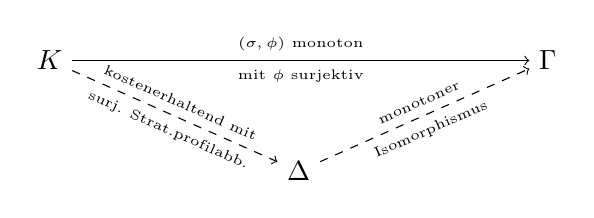
\begin{tikzpicture}
		\node[] 									(K) 	{$K$};
		\node[right of=K, node distance=9em] 		(topM) 	{};
		\node[right of=topM, node distance=9em] 	(Gamma) {$\Gamma$};
		\node[below of=topM, node distance=4em] 	(Delta) {$\Delta$};
		
		\draw[->] (K) --node[above] {\tiny $(\sigma, \phi)$ monoton} node[below] {\tiny mit $\phi$ surjektiv} (Gamma);
		\draw[->, dashed] (K) --node[above, sloped] {\tiny kostenerhaltend mit} node[below, sloped] {\tiny surj. Strat.profilabb.} (Delta);
		\draw[->, dashed] (Delta) --node[above, sloped] {\tiny monotoner} node[below, sloped] {\tiny Isomorphismus} (Gamma);
		\end{tikzpicture}
		\caption{Die in diesem Beweis verwendeten Spiele und Morphismen.}
	\end{figure}		
	Seien also $\Gamma = (I, X, (c_i))$  und $K = (\set{\ast}, Z_\ast, (e_\ast))$ die gegebenen Spiele und $f_i: \IR \to \IR$ die (bijektiven) Kostenabbildungen zu $(\sigma, \phi)$. Dann definieren wir $\Delta \coloneqq (I, X, (f_i^{-1}\circ c_i)_{i \in I})$. Nun hat $(\sigma, \phi): K \to \Delta$ nach Voraussetzung eine surjektive Strategieprofilabbildung und ist ferner kostenerhaltend, denn für jedes $z \in Z_\ast$ gilt:
		\[f_i^{-1}\circ c_i \circ \phi(z) = f_i^{-1} \circ f_i \circ e_\ast(z) = e_\ast(z) = e_{\sigma(i)}(z) \]
	Weiter sind $(\id, \id): \Delta \to \Gamma$ und die Umkehrabbildung $(\id, \id): \Gamma \to \Delta$ monoton, denn
	\begin{center}
		\begin{tikzcd}
			X \arrow[r, "\id"] \arrow[d, "f_i^{-1}\circ c_i"'] 	& X \arrow[d, "c_i"] \\
			\IR \arrow[r, "f_i"]								& \IR
		\end{tikzcd}
			und
		\begin{tikzcd}
			X \arrow[d, "f_i^{-1}\circ c_i"'] 	& X \arrow[l, "\id"] \arrow[d, "c_i"] \\
			\IR 								& \IR \arrow[l, "f_i^{-1}"]
		\end{tikzcd}
	\end{center}		
	kommutieren offenbar. Also sind $\Delta$ und $\Gamma$ tatsächlich monoton isomorph.
\end{proof}

Dies ist also ein Beispiel dafür, wie man eine hinreichende Bedingung für die Existenz eines Potentials durch die Existenz eines passenden Isomorphismus zu einem Koordinationsspiel ausdrücken kann. Allerdings ist die Verträglichkeitsbedinung an monotone Morphismen noch zu stark um auf diesem Weg auch eine notwendige Bedingung für die Existenz eines skalierten Potentials zu erhalten. Dies liegt daran, dass hier eine globale Montonie gefordert wird, während die meisten Potentiale lediglich lokale Monotonie benötigen.

\todo[inline]{Beispiel für die Nicht-Notwendigkeit finden!}

Wir schränken daher die Verträglichkeitsbedingung auf Nachbarschaften ein und kommen so zum Begriff eines skalierten Morphismus. Analog hierzu lassen sich auch für die anderen Potentialbegriffe passende Begriffe eines Morphismus (und damit eines Isomorphismus) definieren - wie das etwa \citeauthor{ReprOfFiniteGamesAsNCG} in \cite[Abschnitt 2.1]{ReprOfFiniteGamesAsNCG} für exakte Potentiale tut\footnote{\citeauthor{ReprOfFiniteGamesAsNCG} bezeichnet zwei exakt isomorphe dann als \glqq ähnlich\grqq.}.

\begin{defn}\label{def:PotentialMorphismen}
	Ein Morphismus $(\sigma, \phi)$ von $\Gamma = (I, X, (c_i)_{i\in I})$ nach $\Delta = (J, Y, (d_j)_{j\in J})$ heißt
	\begin{itemize}
		\item \emph{exakt}, wenn für alle Strategieprofile $x \in X$, Spieler $j \in J$ und Strategien $\hat{x}_{\sigma(j)}$ gilt:
		\[c_{\sigma(j)}(x) - c_{\sigma(j)}(x \mid \hat{x}_{\sigma(j)}) = d_j(\phi(x)) - d_j(\phi(x \mid \hat{x}_{\sigma(j)}))\]
		\item \emph{gewichtend}, wenn es einen Vektor $(w_j)_{j \in J} \in \IR_{\geq 0}^J$ gibt, sodass für alle Strategieprofile $x \in X$, Spieler $j \in J$ und Strategien $\hat{x}_{\sigma(j)}$ gilt:
		\[c_{\sigma(j)}(x) - c_{\sigma(j)}(x \mid \hat{x}_{\sigma(j)}) = w_j\cdot\left(d_j(\phi(x)) - d_j(\phi(x \mid \hat{x}_{\sigma(j)}))\right)\]
		\item \emph{skalierend}, wenn es streng monotone Funktionen $f_j$ gibt, sodass für alle Strategieprofile $x \in X$, Spieler $j \in J$ und Strategien $\hat{x}_{\sigma(j)}$ gilt:
		\[c_{\sigma(j)}(x) - c_{\sigma(j)}(x \mid \hat{x}_{\sigma(j)}) = f_j(d_j(\phi(x))) - f_j(d_j(\phi(x \mid \hat{x}_{\sigma(j)})))\]
		\item \emph{ordinal}, wenn für alle Strategieprofile $x \in X$, Spieler $j \in J$ und Strategien $\hat{x}_{\sigma(j)}$ gilt:
		\[c_{\sigma(j)}(x) < c_{\sigma(j)}(x \mid \hat{x}_{\sigma(j)}) \implies d_j(\phi(x)) < d_j(\phi(x \mid \hat{x}_{\sigma(j)}))\]
		Gilt die Implikation auch in die umgekehrte Richtung, so bezeichnen wir den Morphismus als \emph{biordinal}.
		\item \emph{beste Antwort-erhaltend}, wenn für alle Spieler $j \in J$ und Strategieprofile $x \in X$ gilt:
		\[\phi_j(\arg \min_{x'_{\sigma(j)} \in X_{\sigma(j)}}c_{\sigma(j)}(x' \mid x_{\sigma(j)})) \subseteq \arg \min_{y_j \in Y_j} d_j(\phi(x) \mid y_j)\]
	\end{itemize}	
	Ein exakter/gewichteter/\dots{} Morphismus heißt \emph{exakter/gewichteter/\dots{} Isomorphismus}, wenn er ein Isomorphismus ist und der inverse Morphismus ebenfalls exakt/gewichtet/\dots{} ist.
\end{defn}

\begin{bem}
	Ist ein Morphismus exakt/gewichtet und ein Isomorphismus so ist er automatisch ein exakter/gewichteter Isomorphismus (analog etwa zu Gruppenhomomorphismen). Bei skalierenden\todo{Ist das so? Dann im Satz zur Charakterisierung von Potentialen durch Morphismen Iso streichen.}, ordinalen oder Beste-Antwort-Morphismen muss zusätzlich geprüft werden, ob auch der inverse Morphismus ordinal bzw. Beste-Antwort ist (analog beispielsweise zu stetigen Abbildungen).
\end{bem}

\begin{bsp}
	Betrachte die Spiele 
		\[\Gamma \coloneqq (\set{\ast}, \set{t, b}, (c_\ast)) \text{ mit } c_\ast(t) \coloneqq 0, c_\ast(b) \coloneqq 0\]
	und 
		\[\Delta \coloneqq (\set{\ast}, \set{t, b}, (d_\ast)) \text{ mit } d_\ast(t) \coloneqq 0, d_\ast(b) \coloneqq 1.\]
	Dann ist $(\id, \id): \Gamma \to \Delta$ ein ordinaler, aber kein Beste-Antwort-Morphismus, während $(\id, \id): \Delta \to \Gamma$  ein Beste-Antwort-, aber kein ordinaler Morphismus ist.
\end{bsp}

Während, wie man leicht zeigen kann, die Verknüpfung zweier kostenerhaltender Morphismen wieder einen kostenerhaltenden Morphismus ergibt und die zweier monotoner wieder einen monotonen, ist dies bei exakten/gewichteten/\dots{} Morphismen im Allgemeinen nicht der Fall: 

\begin{bsp}\label{bsp:GegenbspKompositionVMorphismen}
	Betrachte die folgenden drei 1- bzw. 2-Personenspiele:
	\begin{itemize}
		\item $\Gamma \coloneqq (\set{1}, \set{t, b}, c_1)$, wobei die Kostenfunktion $c_1$ wie folgt definiert ist: 
			\[c_1(t) = 0, c_1(b) = 1\]
		\item $\Delta \coloneqq (\set{1, 2}, \set{t, b} \times \set{l, r}, (d_1, d_2))$ mit Kostenfunktionen definiert durch folgende Auszahlungsmatrix (mit Einträgen $(d_1(\_), d_2(\_))$:
		\begin{center}
				\begin{tabular}{c||c|c}
					& l 		& r 		\\\hline\hline
				t	& $(0,0)$	& $(1,0)$	\\\hline
				b	& $(0,1)$	& $(1,1)$ 
			\end{tabular}
		\end{center}
		\item $\Epsilon \coloneqq (\set{1, 2}, \set{t, b} \times \set{l, r}, (e_1, e_2))$ mit Kostenfunktionen definiert durch folgende Auszahlungsmatrix (mit Einträgen $(e_1(\_), e_2(\_))$:
		\begin{center}
			\begin{tabular}{c||c|c}
				& l 		& r 		\\\hline\hline
			t	& $(1,1)$	& $(0,1)$	\\\hline
			b	& $(1,0)$	& $(0,0)$ 
			\end{tabular}
		\end{center}
	\end{itemize}
	Dann sind sowohl die Abbildung $(\sigma, \phi): \Gamma \to \Delta$ mit $\sigma(1) = \sigma(2) = 1$ und $\phi_1(t) = t, \phi_1(b) = b, \phi_2(t) = l, \phi_2(b) = r$ als auch die Abbildung $(\tau, \psi): \Delta \to \Epsilon$ mit $\tau = \id$ und $\psi_i = \id$ exakt, wie man durch einfaches Nachprüfen der jeweiligen Bedingungen sieht. Gleichzeitig ist aber die Verknüpfung der beiden Abbildungen $(\tau, \psi)\circ(\sigma, \phi) = (\sigma\circ\tau, \psi\circ\phi)$ nicht einmal ordinal, denn es gilt
		\[c_{\sigma\circ\tau(1)}(t) = c_1(t) = 0 < 1 = c_1(b) = c_{\sigma\circ\tau(1)}(b) = c_{\sigma\circ\tau(1)}(t \mid b),\]
	aber gleichzeitig
		\[e_1(\psi\circ\phi(t)) = e_1(t,l) = 1 > 0 = e_1(b,r) = e_1(\psi\circ\phi(b)) = e_1(\psi\circ\phi(t \mid b)).\]
\end{bsp}

Insbesondere erhält man also keine Kategorie von Spielen im Sinne der Kategorientheorie, wenn man sich nur auf exakte/gewichtete/\dots{} Morphismen beschränkt (was für kostenerhaltende/monotone Morphismen der Fall ist). Man kann allerdings sicherstellen, dass die Komposition zweier exakter/gewichteter/ordinaler/Beste-Antwort-Morphismen wieder die jeweilige Eigenschaft hat, wenn man sich auf Morphismen mit injektiver Spielerabbildung beschränkt:

\begin{lemma}\label{lemma:KompositionVonMorphismen}
	Die Verknüpfung zweier exakter/gewichteter/ordinaler/Bester-Antwort-Morphismen mit injektiven Spielerabbildungen ist wieder ein solcher Morphismus.
\end{lemma}

\begin{proof}
	Die Aussage des Lemmas ergibt sich aus folgender Beobachtung: Für einen Morphismus $(\sigma, \phi): \Gamma \to \Delta$ mit injektiver Spielerabbildung gilt für jeden Spieler $j$, jedes Strategieprofil $x$ und jede Strategie $\hat{x}_{\sigma(j)}$ von Spieler $\sigma(j)$
		\begin{align}\label{eq:StrategiewechselFuerInjektiveSpielerabbildung}
			\phi(x \mid \hat{x}_{\sigma(j)}) = (\phi(x) \mid \phi_{j}(\hat{x}_{\sigma(j)})).
		\end{align}
	Die Injektivität der Spielerabbildung stellt nämlich gerade sicher, dass die Strategie von Spieler $\sigma(j)$ ausschließlich die Strategie von Spieler $j$ und keinem anderen beeinflusst.
	
	Wir zeigen das Lemma nun für exakte Morphismen - der Beweis für die anderen Morphismenarten geht dann völlig analog. Seien also zwei exakte Morphismen mit injektiver Spielerabbildung gegeben:
		\begin{center}\begin{tikzcd}
			  \Gamma = (I, X, (c_i)) \arrow[r, "{(\sigma, \phi)}"] \arrow[rr, bend right=15, "{(\sigma\circ\tau, \psi\circ\phi)}"'] 
			  & \Delta = (J, Y, (d_j)) \arrow[r, "{(\tau, \psi)}"] 
			  & E 	 = (K, Z, (e_k))
		\end{tikzcd}\end{center}
	Dann ist auch die Verknüpfung der beiden Morphismen exakt, denn es gilt:
		\begin{align*}
			e_k(\psi\circ\phi(x)) &- e_k(\psi\circ\phi(x \mid \hat{x}_{\sigma\circ\tau(k)})) = \\
				&\,\overset{\eqref{eq:StrategiewechselFuerInjektiveSpielerabbildung}}{=}\,\,\,
					e_k(\psi(\phi(x))) - e_k(\psi(\phi(x) \mid \phi_{\tau(k)}(\hat{x}_{\sigma(\tau(k))}))) = \\
				&\!\underset{\text{exakt}}{\overset{(\tau, \psi)}{=}}\,
					d_{\tau(k)}(\phi(x)) - d_{\tau(k)}(\phi(x) \mid \phi_{\tau(k)}(\hat{x}_{\sigma(\tau(k))})) = \\
				&\,\overset{\eqref{eq:StrategiewechselFuerInjektiveSpielerabbildung}}{=}\,\,\, 
					d_{\tau(k)}(\phi(x)) - d_{\tau(k)}(\phi(x \mid \hat{x}_{\sigma(\tau(k))})) = \\
				&\!\underset{\text{exakt}}{\overset{(\sigma, \phi)}{=}}\, 
					c_{\sigma(\tau(k))}(x) - c_{\sigma(\tau(k))}(x \mid \hat{x}_{\sigma(\tau(k))})
				\qedhere
		\end{align*}
\end{proof}

Lediglich bei skalierten Morphismen ist die Komposition zweier solcher auch in diesem Fall und sogar für bijektive Spieler- und Strategieabbildungen im Allgemeinen nicht wieder skaliert, wie das folgende Beispiel zeigt:

\begin{bsp}\label{bsp:GegenbspKompositionSkMorphismen}
	Betrachte die folgenden drei 2-Personenspiele:
	\begin{center}
		$\Gamma:$ \quad
		\begin{tabular}{c||c|c}
			& l 		& r 		\\\hline\hline
		t	& $(0,0)$	& $(0,0)$	\\\hline
		b	& $(1,0)$	& $(2,0)$ 
		\end{tabular}\hspace{3em}
		$\Delta:$ \quad
		\begin{tabular}{c||c|c}
			& l 		& r 		\\\hline\hline
		t	& $(0,0)$	& $(2,0)$	\\\hline
		b	& $(1,2)$	& $(4,2)$ 
		\end{tabular}\hspace{3em}
		$\Epsilon:$ \quad
		\begin{tabular}{c||c|c}
			& l 		& r 		\\\hline\hline
		t	& $(0,0)$	& $(0,0)$	\\\hline
		b	& $(1,1)$	& $(1,1)$ 
		\end{tabular}
	\end{center}
	Dann ist die Abbildung $(\id, \id): \Gamma \to \Delta$ ein skalierter Morphismus mit Skalierungsfunktionen $f_1 \coloneqq \id$ und $f_2 \coloneqq \id$.\todo{Weiter - evtl. gehen die Morphismen gerade in die falsche Richtung?}
\end{bsp}


Da der in \Cref{bsp:Koordinationsspiel} zur Charakterisierung von Koordinationsspielen verwendete Morphismus gerade keine injektive Spielerabbildung verwendet, können die Morphismenbegriffe aus \Cref{def:PotentialMorphismen} nicht dazu verwendet werden um eine zu \Cref{kor:skalPotWennMon1PerMorph} analoge Bedingung für die Existenz der verschiedenen Potentiale zu finden. Dafür erhalten wir aber eine stärkere Form von \Cref{prop:MonIsoKoordDannskPot} zur Charakterisierung von Potentialen:

\begin{prop}\label{prop:CharPotentialeDurchIsos}
	Ein Spiel $\Gamma$ besitzt genau dann ein exaktes/gewichtetes/skaliertes/ordinales/Beste-Antwort-Potential, wenn es exakt/gewichtet/ordinal/Beste-Antwort-isomorph zu einem Koordinationsspiel ist. Es besitzt genau dann ein skaliertes/verallgemeinertes ordinales Potential, wenn es einen skalierten/ordinalen Morphismus mit bijektiven Spieler- und Strategieabbildungen von $\Gamma$ in ein Koordinationsspiel gibt.
\end{prop}

\begin{proof}
	Besitzt ein Spiel $\Gamma= (I, X, (c_i))$ ein exaktes/gewichtetes/skaliertes/ordinales/Beste-Antwort-Potential $P$, so definieren wir das Koordinationsspiel $K = (I, X, (P))$. Dieses ist offenbar isomorph zu $\Gamma$ mittels des Identitätsmorphismus, wobei sich die entsprechende Eigenschaft des Morphismus aus der des Potentials ergibt.
	
	Ist umgekehrt $(\sigma, \phi): \Gamma \to K$ ein exakter/gewichteter/skalierter/ordinaler/Beste-Antwort-Isomorphismus von $\Gamma$ in ein Koordinationsspiel mit einheitlicher Kostenfunktion $p$, dann ist $P \coloneqq p \circ \phi$ ein entsprechendes Potential auf $\Gamma$.
	
	Analog beweist man die Aussage für verallgemeinerte ordinale Potentiale.
\end{proof}

\begin{kor}\label{kor:PotentialeDurchIsosUebertragen}
	Ist ein Spiel $\Gamma$ exakt/gewichtet/skaliert/ordinal/Beste-Antwort-isomorph zu einem Spiel $\Delta$ mit exaktem/gewichtetem/skaliertem/ordinalen/Beste-Antwort-Potential, so hat auch $\Gamma$ selbst ein entsprechendes Potential.
\end{kor}

\begin{proof}
	Nach \Cref{prop:CharPotentialeDurchIsos} ist $\Delta$ exakt/gewichtet/\dots{} isomorph zu einem Koordintionsspiel und da wir laut \Cref{lemma:KompositionVonMorphismen} Isomorphismen verknüpfen können, gilt dies auch für $\Gamma$, welches damit - erneut nach \Cref{prop:CharPotentialeDurchIsos} - ein exaktes/gewichtetes/\dots{} Potential besitzt.
\end{proof}


\subsection{Beweise der Potentialsätze}\label{sec:Morphismen:Potentialsaetze}

Wie wir gesehen haben hängen die verschiedenen Morphismen (und insbesondere Isomorphismen) eng mit den entsprechenden Potentialen zusammen. In diesem Kapitel werden wir dies ausnutzen um mit Hilfe der analogen Eigenschaften der Morphismen die Aussagen aus \Cref{sec:Potentiale} zu zeigen (insbesondere \Cref{satz:ZusammenaengePotentiale}).

\begin{prop}
	Es gelten folgende Beziehungen zwischen den verschiedenen Morphismenbegriffen:
	\begin{center}
		\begin{tikzpicture}
		\node[] (ke) {kostenerhaltend};
		\node[right of=ke, node distance=7em] (ex) {exakt};
		\node[right of=ex, node distance=7em] (gew) {gewichtet};
		\node[right of=gew, node distance=7em] (sk) {skaliert};
		\node[right of=sk, node distance=7em] (ord) {ordinal};
		
		\node[above of=gew, node distance=2em] (mon) {monoton};
		
		\draw[-implies, double equal sign distance] (ke) -- (ex);
		\draw[-implies, double equal sign distance] (ex) -- (gew);
		\draw[-implies, double equal sign distance] (gew) -- (sk);
		\draw[-implies, double equal sign distance] (sk) -- (ord);
		\draw[-implies, double equal sign distance] (ke) -- (mon.west);
		\end{tikzpicture}
	\end{center}
	Für die entsprechenden Isomorphismen gilt sogar:
	\begin{center}
		\begin{tikzpicture}
		\node[] (ke) {kostenerhaltend};
		\node[right of=ke, node distance=6em] (ex) {exakt};
		\node[right of=ex, node distance=5em] (gew) {gewichtet};
		\node[right of=gew, node distance=6em] (sk) {skaliert};
		\node[right of=sk, node distance=5em] (ord) {ordinal};
		\node[right of=ord, node distance=6em] (BA) {Beste Antwort};
				
		\node[above of=gew, node distance=2em] (mon) {monoton};
		
		\draw[-implies, double equal sign distance] (ke) -- (ex);
		\draw[-implies, double equal sign distance] (ex) -- (gew);
		\draw[-implies, double equal sign distance] (gew) -- (sk);
		\draw[-implies, double equal sign distance] (sk) -- (ord);
		\draw[-implies, double equal sign distance] (ke) -- (mon.west);
		\draw[-implies, double equal sign distance] (mon.east) -- (sk);
		\draw[-implies, double equal sign distance] (ord) -- (BA);
		\end{tikzpicture}
	\end{center}
\end{prop}

\begin{proof}
	Die meisten der Folgerungen ergeben sich direkt aus den Definitionen. Für die Morphismen ist:
	\begin{description}
		\item[kostenerh. $\bm{\Rightarrow}$ exakt:] klar
		\item[kostenerh. $\bm{\Rightarrow}$ monoton:] mit Kostenabbildungen $\id: \IR \to \IR$
		\item[exakt $\bm{\Rightarrow}$ gew:] mit Gewichten $w_j \coloneqq 1$
		\item[gew $\bm{\Rightarrow}$ skaliert:] $f_j: \IR \to \IR: t \mapsto w_j \cdot t$ sind streng monotone Skalierungsfunktionen.
		\item[skaliert $\bm{\Rightarrow}$ ordinal:] Gilt $c_{\sigma(j)}(x) < c_{\sigma(j)}(x \mid \hat{x}_{\sigma(j)})$ so auch $f_j \circ d_j(\phi(x)) < f_j \circ d_j(\phi(x \mid \hat{x}_{\sigma(j)}))$ und (wegen strenger Monotonie von $f_j$) $d_j(\phi(x)) < d_j(\phi(x \mid \hat{x}_{\sigma(j)}))$.
	\end{description}
	Die zusätzlichen Zusammenhänge von Isomorphismen sind:
	\begin{description}
		\item[monoton $\bm{\Rightarrow}$ skaliert:] mit dem gleichen Beweis wie \Cref{prop:MonIsoKoordDannskPot} (wir haben dabei nirgends verwendet, dass eines der beteiligten Spiele ein Koordinationsspiel ist)
		\item[skaliert $\bm{\Rightarrow}$ BA:] Ist $(\sigma, \phi)$ ein skalierter Isomorphismus, so gilt 
			\[c_{\sigma(j)}(x) < c_{\sigma(j)}(x \mid \hat{x}_{\sigma(j)}) \iff f_j \circ d_j(\phi(x)) < f_j \circ d_j(\phi(x \mid \hat{x}_{\sigma(j)})) \iff d_j(\phi(x)) < d_j(\phi(x \mid \hat{x}_{\sigma(j)})).\]
		Da sowohl $\phi_j$ als auch $\sigma$ bijektiv sind, folgt damit bereits, dass $(\sigma, \phi)$ auch ein Beste-Antwort-Isomorphismus ist. \qedhere
	\end{description}	
\end{proof}

Mit \Cref{prop:CharPotentialeDurchIsos} erhalten wir aus der vorherigen Proposition einen Großteil der in \Cref{diag:Potentiale} dargestellten Beziehungen zwischen den verschiedenen Potentialbegriffen. Es bleibt noch zu zeigen, dass Beste-Antwort-Potentiale lokale Nash und verallgemeinert ordinale Potentiale verallgemeinert Nash sind. Dies werden wir erneut aus allgemeineren Sätzen über ordinale bzw. Beste-Antwort-Morphismen folgern.

Wie wir bereits in \Cref{beob:VerbPfadeundNGe} gesehen haben, hängen Nash-Gleichgewichte eng mit (abgeschlossenen) Verbesserungspfaden zusammen. Wir zeigen daher zunächst wie diese sich mit ordinalen Morphismen vertragen.

\begin{prop}\label{prop:NVReflVerbErh}
	Sei $(\sigma, \phi): \Gamma \to \Delta$ ein ordinaler Morphismus mit surjektiver Spielerabbildung $\sigma$ und $\gamma = (x^0, x^1, \dots)$ ein Pfad in $X$, sodass auch $\phi(\gamma) \coloneqq (\phi(x^0), \phi(x^1), \dots)$ ein Pfad in $Y$ ist. Ist dann $\phi(\gamma)$ ein Nicht-Verschlechterungspfad, so auch $\gamma$. Ist $\gamma$ sogar ein Verbesserungspfad, so auch $\phi(\gamma)$.
\end{prop}

Ordinale Morphismen mit surjektiver Spielerabbildung erhalten also Verbesserungspfade und reflektieren Nicht-Verschlechterungspfade. Daraus folgt dann insbesondere \Cref{prop:ordPotVerbpfad}, der dies für (verallgemeinerte) ordinale Potentiale behauptet.

\begin{proof}
	Sei zunächst $\phi(\gamma)$ ein Nicht-Verschlechterungspfad. Angenommen $\gamma$ wäre kein Nicht-Verschlechterungspfad, dann gäbe es also ein $k$, sodass sich der im $k$-ten Schritt abweichende Spieler echt verschlechtert, d.h. $c_{i(k)}(x^k) > c_{i(k)}(x^{k-1})$. Da $\sigma: J \to I$ surjektiv ist, gibt es nun einen Spieler $j \in J$ mit $\sigma(j) = i(k)$ und wegen der Ordinalität von $\phi$ gilt für diesen, dass er sich im $k$-ten Schritt von $\phi(\gamma)$ echt verschlechtert, d.h. $d_j(\phi(x^k)) > d_j(\phi(x^{k-1}))$. 
	
	Insbesondere wissen wir damit, dass es auch in $\phi(\gamma)$ einen Spieler $j(k)$ geben muss, der im $k$-ten Schritt seine Strategie echt ändert. Damit gilt
		\[\phi_{\sigma(j(k))}\left(x_{\sigma(j(k))}^k\right) = \left(\phi(x^k)\right)_{\sigma(j(k))} \neq \left(\phi(x^{k-1})\right)_{\sigma(j(k))} = \phi_{\sigma(j(k))}\left(x_{\sigma(j(k))}^{k-1}\right)\]
	Daraus folgt $x_{\sigma(j(k))}^k \neq x_{\sigma(j(k))}^{k-1}$ und, da es in einem Pfad pro Schritt höchstens einen abweichenden Spieler geben kann, auch $i(k) = \sigma(j(k))$. Aus der Ordinalität von $\phi$ folgt dann aber aus $c_{i(k)}(x^k) > c_{i(k)}(x^{k-1})$, dass sich aus $j(k)$ echt verschlechtert, d.h. $d_{j(k)}(\phi(x^k)) > d_{j(k)}(\phi(x^{k-1}))$ - im Widerspruch dazu, dass $\phi(\gamma)$ ein Nicht-Verschlechterungspfad ist.

	Ist nun $\gamma$ ein Verbesserungspfad, gilt in jedem Schritt $c_{i(k)}(x^{k}) < c_{i(k)}(x^{k-1})$ und daher - mit dem gleichen Argument wie eben - auch $d_{j(k)}(\phi(x^{k+1})) < d_{j(k)}(\phi(x^k))$. Also ist auch $\phi(\gamma)$ ein Verbesserungspfad.
\end{proof}

Im Allgemeinen bilden (ordinale) Morphismen Pfade nicht wieder auf Pfade ab. Ist nämlich $(\sigma, \phi): \Gamma \to \Delta$ ein solcher Morphismus und gibt es zwei Spieler $j$ und $j'$ mit $\sigma(j) = \sigma(j') \eqqcolon i$, dann kann eine einseitige Abweichung von Spieler $i$ in $\Gamma$ zu einer gleichzeitigen Abweichung der \emph{beiden} Spieler $j$ und $j'$ in $\Delta$ führen. Wie wir bereits im Beweis von \Cref{lemma:KompositionVonMorphismen} gesehen haben, kann dies allerdings nicht passieren, wenn die Spielerabbildung $\sigma$ injektiv ist.

\begin{beob}\label{beob:PfadeAufPfade}
	Morphismen $(\sigma, \phi)$ mit injektivem $\sigma$ bilden Pfade auf Pfade ab.
\end{beob}

Dies erlaubt uns folgendes Korollar:

\begin{kor}\label{kor:ReflAbg}
	Sei $(\sigma, \phi): \Gamma \to \Delta$ ein ordinaler Morphismus mit bijektiver Spielerabbildung $\sigma$ und $\gamma = (x^0, \dots, x^n)$ ein Verbesserungspfad in $X$. Ist dann $\phi(\gamma)$ abgeschlossen in $\Delta$, so ist auch $\gamma$ in $\Gamma$ abgeschlossen.
\end{kor}
	
\begin{proof}	
	Nehmen wir im Widerspruch zur Behauptung an, $\gamma$ wäre nicht abgeschlossen. Dann gäbe es folglich ein Strategieprofil $x^{n+1} \in X$, welches $\gamma$ zu einem Verbesserungspfad $\gamma' \coloneqq (x^0, \dots, x^n, x^{n+1})$ in $\Gamma$ verlängert. Nach \Cref{beob:PfadeAufPfade} ist dann auch $\phi(\gamma')$ ein Pfad in $\Delta$ und mit \Cref{prop:NVReflVerbErh} sogar ein Verbesserungspfad, also insbesondere eine Verlängerung des Pfades $\phi(\gamma)$ - ein Widerspruch zu dessen Abgeschlossenheit.
\end{proof}

\begin{kor}\label{kor:ReflektNG}
	Ordinale Morphismen mit bijektiver Spielerabbildung reflektieren Nash-Gleichgewichte. Das heißt, ist $x \in X$ ein Strategieprofil in $\Gamma$ und $(\sigma, \phi)$ ein ordinaler Morphismus in ein Spiel $\Delta$, sodass $\phi(x)$ ein Nash-Gleichgewicht in diesem ist, dann war bereits $x$ ein Nash-Gleichgewicht von $\Gamma$.
\end{kor}

\begin{proof}
	Es ist $x$ ein trivialer Verbesserungspfad in $\Gamma$, dessen Bild $\phi(x)$ in $\Delta$ abgeschlossen ist. Daher ist mit \Cref{kor:ReflAbg} $x$ in $\Gamma$ abgeschlossen und folglich (vgl. \Cref{beob:VerbPfadeundNGe}) $x$ ein Nash-Gleichgewicht in $\Gamma$.
\end{proof}

\todo[inline]{Zu obigen Sätzen jeweils Beispiele für Notwendigkeit der Voraussetzungen finden}

Aus diesem Korollar folgt insbesondere, dass Nash-Gleichgewichte in von einem verallgemeinerten ordinalen Potential induzierten Koordinationsspiel auch Nash-Gleichgewichte im Ausgangsspiel sind. Also sind verallgemeinerte ordinale Potentiale verallgemeinerte Nash-Potentiale.

\begin{bsp}
	Ordinale Isomorphismen haben insbesondere injektive Spieler- und Strategieabbildungen. Damit erfüllen sie die Voraussetzungen von \Cref{kor:ReflektNG}, d.h. ordinal isomorphe Spiele haben die gleichen Nash-Gleichgewichte.
\end{bsp}

Dies zeigt also nochmal, dass ordinale Potentiale lokale Nash-Potentiale sind. Es verbleibt die entsprechende Aussage für Beste-Antwort-Potentiale. Dazu betrachten stellen wir zunächst fest, dass Beste-Antwort-Morphismen mit bijektiver Spielerabbildung Beste-Antwort-Schritte (und damit auch -Pfade und Nash-Gleichgewichte) erhalten.

\begin{prop}\label{prop:BAMorphErhBASchritte}
	Sei $(\sigma, \phi): \Gamma \to \Delta$ ein Beste-Antwort-Morphismus mit bijektiver Spielerabbildung $\sigma$ und $(x^0, x^1)$ ein Beste-Antwort-Schritt von Spieler $\sigma(i)$ in $\Gamma$, so auch $\phi((x^0, x^1))$ von Spieler $i$ in $\Delta$.
\end{prop}

\begin{proof}
	Da $\sigma$ bijektiv ist, können wir ohne Einschränkung annehmen, dass $\sigma$ die Identität ist. Ferner wissen wir damit, dass aus $x^1 = (x^0 \mid x^1_i)$ auch $\phi(x^1) = \phi((x^0 \mid x^1_i)) = (\phi((x^0) \mid \phi_i(x^1_i)$ folgt. Da dieser Schritt sogar ein Bester-Antwort-Schritt ist, gilt $x^1_i \in \arg\max_{x_i \in X_i} c_i(x^0 \mid x_i)$ und daher mit der definierenden Eigenschaft von Beste-Antwort-Morphismen auch $\phi_i(x^1_i) \in \arg\max_{y_i \in Y_i} d_i(\phi(x^0) \mid y_i)$. Also ist $\phi((x^0, x^1))$ ebenfalls ein Beste-Antwort-Schritt (von Spieler $i$).
\end{proof}

\begin{kor}
	Beste-Antwort-Morphismus mit bijektiver Spielerabbildung bewahren Besten-Antwort-Pfade und Nash-Gleichgewichte.
\end{kor}

\begin{proof}
	Der erste Teil der Aussage ergibt sich direkt aus der vorangegangenen \Cref{prop:BAMorphErhBASchritte}. Sei also $x$ ein Nash-Gleichgewicht von $\Gamma$, dann ist $(x,x)$ ein Beste-Antwort-Schritt für alle Spieler $i \in I$. Damit ist $(\phi(x), \phi(x))$ ebenfalls ein Beste-Antwort-Schritt für jeden Spieler und daher insbesondere ein Nash-Gleichgewicht (vgl. \Cref{beob:BASchritteNG}).
\end{proof}

Beste-Antwort-isomorphe Spiele haben damit sogar die gleichen Nash-Gleichgewichte, womit Beste-Antwort-Potentiale lokale Nash-Potentiale sind. Außerdem folgt hieraus \Cref{prop:BAPotBAPfad}, sodass wir nun den Beweis von \Cref{satz:ZusammenaengePotentiale} vervollständigt haben.


\subsection{Weitere Sätze mit Morphismen}

Zum Abschluss dieses Kapitels wollen wir nun noch einige weitere Beobachtungen über bzw. mit Morphismen festhalten:

Für monotone Morphismen gibt es einen zu \Cref{prop:NVReflVerbErh} analogen Satz über Nicht-Verschlechterungs- und Verbesserungspfade.

\begin{prop}
	Sei $(\sigma, \phi): \Gamma \to \Delta$ ein monotoner Morphismus und $\gamma = (x^0, x^1, \dots)$ ein Pfad in $X$, sodass auch $\phi(\gamma) \coloneqq (\phi(x^0), \phi(x^1), \dots)$ ein Pfad in $Y$ ist. Ist dann $\gamma$ ein Nicht-Verschlechterungspfad, so auch $\phi(\gamma)$. Ist $\phi(\gamma)$ sogar ein Verbesserungspfad, so auch $\gamma$.
\end{prop}

Das heißt monotone Morphismen erhalten Nicht-Verschlechterungspfade und reflektieren Verbesserungspfade - also genau umgekehrt zu ordinalen Morphismen.

\begin{proof}
	Zunächst beobachten wir, dass $\sigma$ immer den in $\phi(\gamma)$ im $k$-ten Schritt abweichenden Spieler (sofern es einen solchen gibt) auf den im gleichen Schritt abweichenden Spieler in $\gamma$ abbildet. Ist nämlich $j(k)$ der entsprechende Spieler aus $\Delta$, so gilt:
	\[\phi_{\sigma(j(k))}\left(x_{\sigma(j(k))}^k\right) = \left(\phi(x^k)\right)_{\sigma(j(k))} \neq \left(\phi(x^{k-1})\right)_{\sigma(j(k))} = \phi_{\sigma(j(k))}\left(x_{\sigma(j(k))}^{k-1}\right)\]
	Daraus folgt $x_{\sigma(j(k))}^k \neq x_{\sigma(j(k))}^{k-1}$ und, da es in einem Pfad pro Schritt höchstens einen abweichenden Spieler geben kann, auch $i(k) = \sigma(j(k))$.
	
	Ist nun $\gamma$ ein Nicht-Verschlechterungspfad und es gibt im $k$-ten Schritt einen (echt) abweichenden Spieler $j(k)$, so ist also $\sigma(j(k)) = i(k)$ und daher $c_{\sigma(j(k))}(x^k) \leq c_{\sigma(j(k))}(x^{k-1})$. Mit der Monotonie von $\phi$ folgt daraus direkt auch $d_{j(k)}(\phi(x^k)) \leq d_{j(k)}(\phi(x^{k-1}))$.
	
	Ist $\phi(\gamma)$ ein Verbesserungspfad, gilt in jedem Schritt $d_{j(k)}(\phi(x^{k+1})) < d_{j(k)}(\phi(x^k))$ und daher - erneut wegen der Monotonie von $\phi$ - auch $c_{\sigma(j(k))}(x^{k+1}) < c_{\sigma(j(k))}(x^{k})$.
\end{proof}

Der folgende Satz zeigt, wann man Spieler weglassen kann, ohne dadurch die Nash-Gleichgewichte des Spiels zu beeinflussen.

\begin{satz}\label{prop:DummySpielerWeglassen}
	Sei $(\sigma, \phi): \Gamma \to \Delta$ ein biordinaler Morphismus mit injektiver Spielerabbildung und surjektiven Strateegieabbildungen. Seien ferner alle Spieler in $I\setminus \sigma(J)$ Dummy-Spieler. Dann ist ein Strategieprofil $x \in X$ genau dann ein Nash-Gleichgewicht in $\Gamma$, wenn $\phi(x)$ ein Nash-Gleichgewicht in $\Delta$ ist.
\end{satz}

% \todo[inline]{Kann man das noch schöner ausdrücken (mit Retrakten o.ä.)?}

\begin{proof}
	Sei zunächst $x \in X$ ein Nash-Gleichgewicht in $\Gamma$ und $y_j \in Y_j$. Da $\phi_j$ surjektiv ist, gibt es dann ein $\hat{x}_{\sigma(j)}$ mit $\phi_j(\hat{x}_{\sigma(j)}) = y_j$. Wegen der Injektivität von $\sigma$ gilt ferner $\phi(x \mid \hat{x}_{\sigma(j)}) = \left(\phi(x) \mid y_j\right)$.
	
	Da $x$ ein Nash-Gleichgewicht ist, gilt nun $c_{\sigma(j)}(x) \leq c_{\sigma(j)}(x \mid \hat{x}_{\sigma(j)})$ und folglich wegen der Biordinalität von $\phi$ auch $d_j(\phi(x)) \leq d_j(\phi(x \mid \hat{x}_{\sigma(j)})) = d_j(\phi(x) \mid y_j)$. Also ist auch $\phi(x)$ ein Nash-Gleichgewicht in $\Delta$.
	
	Ist umgekehrt $\phi(x)$ ein Nash-Gleichgewicht in $\Delta$ und $\hat{x}_i$ eine alternative Strategie von Spieler $i \in I$. 
	\begin{description}
		\item[1. Fall:] Liegt $i$ in $I\setminus \sigma(J)$, so ist $i$ nach Voraussetzung ein Dummy-Spieler und folglich gilt: $c_i(x) = c_i(x \mid \hat{x}_i)$.
		\item[2. Fall:] Liegt $i$ hingegen in $\sigma(J)$, so gibt es also einen Spieler $j \in J$ mit $\sigma(j) = i$. Aus der Injektivität von $\sigma$ und dem Wissen, dass $\phi(x)$ ein Nash-Gleichgewicht ist, folgt nun $d_j(\phi(x \mid \hat{x}_i)) = d_j(\phi(x) \mid \phi_j(\hat{x}_{\sigma(j)})) \geq d_j(\phi(x))$. Über die Biordinalität von $\phi$ erhalten wir schließlich $c_i(x \mid \hat{x}_i) = c_{\sigma(j)}(x \mid \hat{x}_i) \geq c_{\sigma(j)}(x) = c_i(x)$. 
	\end{description}
	Insgesamt ist also auch $x$ ein Nash-Gleichgewicht.
\end{proof}

Mit diesem Satz können wir nun die in \Cref{beob:endlicheSpiele} gemachte Beobachtung formalisieren (und beweisen), dass Spieler mit nur einer einzigen Strategie beim Untersuchen von Nash-Gleichgewichten immer ignoriert werden können:

\begin{kor}\label{kor:EinStratSpielerWeglassen}
	Spieler mit nur einer einzigen Strategie können immer entfernt werden ohne die Nash-Gleichgewichte zu verändern.
\end{kor}

\begin{proof}
	Sei dazu $\Gamma$ ein beliebiges Spiel und $I' \subseteq I$ eine solche Teilmenge von Spielern, dass alle Spieler $i$ in $I \setminus I'$ genau eine Strategie $\ast_i$ besitzen. Dann betrachten wir die Einschränkung von $\Gamma$ auf die Spieler in $I'$, nämlich $\Gamma' \coloneqq (I', \prod_{i \in I'}X_i, (c'_i)_{i \in I'})$, wobei die Kostenfunktionen wie folgt definiert sind:
		\[c'_{\hat{\imath}}(x') \coloneqq c_{\hat{\imath}}(x), \text{ wobei $x \in X$ definiert ist durch } x_i = \begin{cases}x'_i, &i \in I'\\ \ast_i, &\text{sonst}\end{cases}\]
	und den folgenden Morphismus $(\sigma, \phi): \Gamma \to \Gamma'$ zwischen den beiden Spielen:
	\begin{align*}
		\sigma:	&&I\setminus I'	\to	 I:	&&i	\mapsto	i  \\
		\phi_i:	&&X_i	\to	 X_i:		&&x_i	\mapsto	x_i
	\end{align*}	
	Dieser ist offenbar kostenerhaltend, also insbesondere biordinal, die Spielerabbildung ist injektiv, die Strategieabbildungen sind surjektiv und $I\setminus \sigma(I') = I \setminus I'$ enthält nur Dummy-Spieler. Damit folgt die Behauptung mit \Cref{prop:DummySpielerWeglassen}.
\end{proof}

Schließlich wollen wir noch eine Verallgemeinerung von \Cref{beob:ZshExGewPot} beweisen:

\begin{lemma}
	Seien $\Gamma = (I, X, (c_i))$ und $\Delta = (J, Y, (d_j))$ zwei Spiele. Dann gibt es genau dann einen gewichteten Morphismus $\Gamma \to \Delta$, wenn es positive Gewichte $(w_j)_{j\in J}$ und einen exakten Morphismus $\Gamma \to \Delta_w \coloneqq (J, Y, (w_j\cdot d_j))$ gibt.
\end{lemma}

\begin{proof}
	Ein Morphismus $(\sigma, \phi): \Gamma \to \Delta$ ist genau dann ein exakter Morphismus zwischen $\Gamma$ und $\Delta_w$, wenn für alle Strategieprofile $x \in X$, Spieler $j \in J$ und Strategien $\hat{x}_{\sigma(j)}$ gilt:
		\[c_{\sigma(j)}(x) - c_{\sigma(j)}(x \mid \hat{x}_{\sigma(j)}) = w_j \cdot d_j(\phi(x)) - w_j \cdot d_j(\phi(x \mid \hat{x}_{\sigma(j)}))\]
	Und dies ist offenbar äquivalent zu
		\[c_{\sigma(j)}(x) - c_{\sigma(j)}(x \mid \hat{x}_{\sigma(j)}) = w_j \cdot \left(d_j(\phi(x)) - d_j(\phi(x \mid \hat{x}_{\sigma(j)}))\right),\]
	also dazu, dass $(\sigma, \phi)$ ein gewichteter Morphismus zwischen $\Gamma$ und $\Delta$ ist.
\end{proof}